% Minimal TikZ standalone example
\documentclass[tikz, border=1mm]{standalone}

\usepackage{amsmath,amssymb}
\usepackage{tikz}
\usepackage{tkz-euclide}

\usetikzlibrary{calc,angles,quotes}

\begin{document}
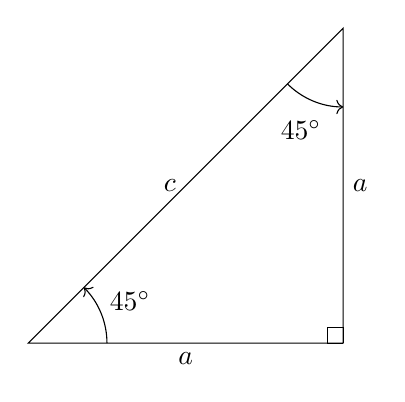
\begin{tikzpicture}[scale=1.0]

	\coordinate (A) at (0,0);
	\coordinate (B) at (4,0);
	\coordinate (C) at (4,4);

	% triangle
	\draw (A) -- (B) -- (C) -- cycle;

	% right angle mark
	\tkzMarkRightAngle[size=0.2](C,B,A)

	% side labels (a opposite A, etc.)
	\node[below] at ($(A)!0.5!(B)$) {$a$};
	\node[left]  at ($(A)!0.5!(C)$) {$c$};
	\node[right] at ($(B)!0.5!(C)$) {$a$};

	% angle labels
	\pic["$45^\circ$", draw, ->, angle eccentricity=1.4, angle radius=1.0cm]
		{angle = B--A--C};
	\pic["$45^\circ$", draw, ->, angle eccentricity=1.4, angle radius=1.0cm]
		{angle = A--C--B};

\end{tikzpicture}
\end{document}
